\chapter{A Framework For The Quasi-classical Model}
\label{ch:basics}

\section{Theory Of Superconductivity}

The discovery of the isotope effect in 1950 revealed that not only lattice electrons but rather the whole lattice determines the superconducting properties of a solid. Experiments measuring the critical temperature $T_c$ of different mercury isotopes showed that, indeed, there is a relation between the isotope mass and $T_c$. Herbert Fr\"ohlich was then the first to introduce a new concept to explain superconductivity. He showed that a phonon-mediated interaction between electrons and the lattice could lead to an attractive long-range interaction of electrons in the lattice. Figuratively speaking, an electron passing through the crystal lattice will polarize it by attracting the positive ions. It leaves a deformed lattice, which will then attract a second electron. An effective attractive interaction between these two electrons is thereby created. % – they form a Cooper pair. 
In 1956, Cooper showed that the electronic ground state, the Fermi sea at $T = 0$, is unstable if a weak attractive interaction is taken into account. This layed the foundation of the BCS theory \cite{Bardeen1957}, the first successful microscopic theory after the discovery of superconductivity in 1911 by Heike Kammerlingh Onnes. 

%TODO maybe include picture that explains, why opposite k vectors

\subsection*{Preliminaries}
The BCS Hamiltonian reads 
\begin{align}
H &= H_0 + H_1 \label{eq:H}\\
H_0 &= \sum_{\mathbf{k}, \sigma} \xi_{\mathbf{k}} c^{\dagger}_{\mathbf{k} \sigma }c_{\mathbf{k} \sigma }  \label{eq:H0}\\
H_1 &= \frac{1}{N} \sum_{\mathbf{k}, \mathbf{k'}} V_\mathbf{{\mathbf{k} \mathbf{k'}}} c^{\dagger}_{\mathbf{k} \uparrow }c^{\dagger}_{- \mathbf{k} \downarrow}   c_{- \mathbf{k'} \downarrow} c_{\mathbf{k'} \uparrow} \label{eq:H1}
\end{align}
The operators $c^\dagger_{\mathbf{k}, \sigma}$ and $c_{\mathbf{k}, \sigma}$ are fermion operators that create or annihilate an electron with momentum $\mathbf{k}$ and spin $\sigma$. The first term in the Hamiltonian $H$ is the unperturbed electron Hamiltonian $H_0$ with parabolic energy dispersion $\xi_{\mathbf{k}}$. The  second term is the interaction Hamiltonian $H_1$, expressing the scattering of two electrons from $(\mathbf{k'} \downarrow,  - \mathbf{k'} \uparrow)$ to $(\mathbf{k} \uparrow , - \mathbf{k} \downarrow)$. The interaction potential $V_\mathbf{{\mathbf{k}, \mathbf{k'}}}$ exchanges the scattering for electrons with energy $|\xi_\mathbf{k}| \lesssim \hbar \omega_D$.
%TODO check!
The Hamiltonian in eq. (\ref{eq:H}) can be simplified by a mean-field approximation. In this approximation, an operator $A$ is expressed by a sum of its statistical mean $\braket{A}$ and small statistical fluctuations $\delta A$. Since the fluctuations are assumed to be small, terms with $\mathcal{O}((\delta A)^2)$ can be neglected.
\begin{align}
A &= \langle A \rangle + \delta A, \quad B = \langle B \rangle + \delta B  \nonumber \\
A B &= \langle A \rangle  \langle B \rangle  + \langle A \rangle  \delta B +  \langle B \rangle \delta A + \underbrace{\delta A \delta B}_{\approx 0}\label{eq:meanfield-der}
\end{align}
Using $\delta A = A - \langle A \rangle$ and inserting this back into eq. (\ref{eq:meanfield-der}) leads to
\begin{equation}
AB = \langle A \rangle B + \langle B \rangle A - \langle A \rangle \langle B \rangle.\label{eq:meanfield-ab}
\end{equation}
This approximation is applied to the interaction part $H_1$ in eq. (\ref{eq:H1}), replacing
\begin{equation}
A = c^{\dagger}_{\mathbf{k} \uparrow }c^{\dagger}_{- \mathbf{k} \downarrow}, \quad B =  c_{- \mathbf{k'} \downarrow} c_{\mathbf{k'} \uparrow} .
\end{equation}
The result is the BCS-Hamiltonian
\begin{equation}
H_{\text{BCS}} = \sum_{\mathbf{k}, \sigma} \xi_{\mathbf{k}} c^{\dagger}_{\mathbf{k} \sigma }c_{\mathbf{k} \sigma }    -  \sum_{\mathbf{k}} \Delta_{\mathbf{k}}^* c_{-\mathbf{k} \downarrow} c_{\mathbf{k} \uparrow}  - \sum_{\mathbf{k}} \Delta_{\mathbf{k}}  c^{\dagger}_{\mathbf{k} \uparrow} c^{\dagger}_{- \mathbf{k} \downarrow} + \text{const.}\label{eq:H-BCS}
\end{equation}
where 
\begin{eqnarray}
\Delta_{\mathbf{k}} &:=& - \frac{1}{N} \sum_{\mathbf{k'}} V_\mathbf{{\mathbf{k} \mathbf{k'}}} \langle c_{-\mathbf{k'} \downarrow} c_{\mathbf{k'} \uparrow} \rangle \\
\Delta_{\mathbf{k}}^* &:=& - \frac{1}{N} \sum_{\mathbf{k'}} V_\mathbf{{\mathbf{k} \mathbf{k'}}}  \langle  c^{\dagger}_{\mathbf{k'} \uparrow} c^{\dagger}_{- \mathbf{k'} \downarrow} \rangle
\end{eqnarray}
%TODO why is this the pair potential?
The BCS-Hamiltonian in eq. (\ref{eq:H-BCS}) can be diagonalized using the Bogoliubov transformation. The aim is to express the Hamiltonian in the basis of new fermion operators. These new operators will describe quasiparticles, which are a linear combination of $c^\dagger_{\mathbf{k}, \sigma}$ and $c_{\mathbf{k}, \sigma}$.
\begin{equation}
\begin{pmatrix}
\gamma_{\mathbf{k} \uparrow} \\ \gamma^{\dagger}_{-\mathbf{k} \downarrow}  
\end{pmatrix} = \begin{pmatrix}
u^*_{\mathbf{k} } & -v_{\mathbf{k} } \\
v^*_{\mathbf{k} }  & u_{\mathbf{k} } 
\end{pmatrix} 
\begin{pmatrix}
c_{\mathbf{k} \uparrow} \\ c^{\dagger}_{-\mathbf{k} \downarrow}  
\end{pmatrix}
\end{equation}\label{eq:bogol-trans}
Evaluating the fermion anticommutation relation using the transformation above yields
\begin{equation}
\left\{ \gamma_{\mathbf{k} \uparrow}, \gamma^{\dagger}_{\mathbf{k} \uparrow}  \right\}  = \dots = |u_{\mathbf{k}}|^2  + |v_{\mathbf{k}}|^2 \stackrel{!}{=} 1
\end{equation}
and will lead to the inverse transformation of eq. (\ref{eq:bogol-trans}). Inserting the inverse transformation into the BCS-Hamiltonian in eq. (\ref{eq:H-BCS}) will give the coefficients $u_{\mathbf{k}}$, $v_{\mathbf{k}}$ from eq. (\ref{eq:bogol-trans}) and finally yield to the diagonalized form of the BCS-Hamiltonian
\begin{equation}
H_{\text{BCS}} =  \sum_{ \mathbf{k} \sigma } E_{ \mathbf{k} } \gamma^{\dagger}_{\mathbf{k} \sigma } \gamma_{\mathbf{k} \sigma }
\end{equation}
\begin{equation}
E_{\mathbf{k}} :=  \sqrt{\xi^2_{\mathbf{k}}  + |\Delta_{\mathbf{k}}|^2 } \label{eq:E-k}
\end{equation}
\begin{figure}
\centering
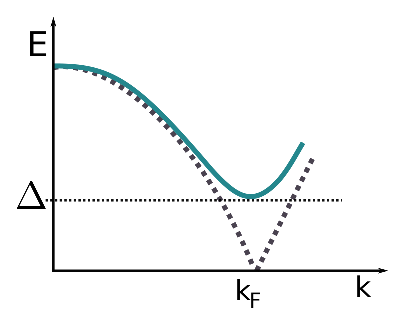
\includegraphics[width=0.5\textwidth]{figure/framework-analytical/bcs-spectrum_csch}
\caption{Excitations from BCS theory. The dashed line is the normal state dispersion relation ($\Delta = 0$). The solid line is the dispersion relation for the superconducting state ($\Delta \neq 0$), where no excitations with energies $\epsilon < \Delta$ are present. } \label{fig:bcs-spectrum}
\end{figure}
For a fixed energy $E_k \stackrel{!}{=} \epsilon $, eq. (\ref{eq:E-k}) gives two possible values for $\xi_k$:
\begin{equation}
\xi_\mathbf{k} = \pm \sqrt{\epsilon^2 - | \Delta_\mathbf{k}|^2}.
\end{equation}
Knowing that $k^2 = k_F^2 \pm 2m\sqrt{\epsilon^2 + |\Delta_k|^2} \hbar^2$, one can calculate the group velocity as 
\begin{equation}
v_g = \frac{d \epsilon}{d (\hbar k)} = \pm v_F \frac{\sqrt{\epsilon^2 - |\Delta|^2}}{\epsilon}.
\end{equation}
The group velocity is positive for excitations outside the Fermi surface and negative for excitations inside. Therefore, the positive solution is a particle-like excitation, and the negative solution is a hole-like excitation. Figure \ref{fig:bcs-spectrum} shows the excitation spectrum of particles and holes from the BCS theory. 

\subsection*{Bogoliubov de Gennes Hamiltonian}
%Motivation for BdG: Describing inhomogneous systems, example Josephson junctions --> need for a microsopic theory for inhomogenous systems. 
%Idea: make BCS- mean field hamiltonian spatially dependent. 
The ansatz for the BCS ground state used by Bardeen, Cooper and Schrieffer is based on the concept of Cooper pairs. It is a direct consequence of the instability in the ground state through the attractive interaction. The BCS theory proposes a BCS ground state built on eigenstates of the single-particle Hamiltonian $H_0$ from eq. (\ref{eq:H0}), leading to a ground state that consists of a linear combination of pair states. %TODO check!
\begin{eqnarray}
\ket{\psi_\text{BCS}} &=& \prod_{ \mathbf{k} } (u_\mathbf{k} + v_\mathbf{k} c^{\dagger}_{ \mathbf{k} \uparrow } c^{\dagger}_{ - \mathbf{k} \downarrow }) \ket{\text{vac}} \\
H_\text{BCS} \ket{\psi_\text{BCS}} &=& E_\text{BCS} \ket{\psi_\text{BCS}}  
\end{eqnarray}
In most cases however, a more realistic set-up or inhomogeneous system cannot be described in terms of eigenfunctions of $H_0$. With a vector potential $\mathbf{A} \neq 0$, for example, time reversal symmetry is not given any more. %TODO Überleitung (“In the general case”)
The characteristic length scale is the superconducting coherence length $\xi_0$. If a system is varying slowly over a length scale $l \approx \xi_0$, a spatially dependent, more general Hamiltonian is needed. 
In order to find an adequate expression for such a spatially dependent Hamiltonian, the following spinor is introduced
\begin{equation}
\ket{\Psi_\mathbf{k}} = \begin{pmatrix}
| \Psi_\mathbf{k_1} \rangle \\ | \Psi_\mathbf{k_2} \rangle
\end{pmatrix} := \begin{pmatrix}
c^{\dagger}_{\mathbf{k}, \uparrow} \\ c_{- \mathbf{k}, \downarrow}
\end{pmatrix} \ket{\psi_\text{BCS}} \label{eq:spinor}
\end{equation}
In this basis $\left\{| \Psi_\mathbf{k_1} \rangle, | \Psi_\mathbf{k_2} \rangle \right\}$, the Hamiltonian (\ref{eq:H-BCS}) takes the form known as the Bogoliubov de Gennes Hamiltonian
\begin{equation}
H_\text{BdG}\left(\mathbf{k} \right) = \begin{pmatrix}
\xi_\mathbf{k} &  - \Delta_\mathbf{k}\\
- \Delta^*_\mathbf{k} & - \xi_\mathbf{k}
\end{pmatrix} \label{eq:H-BdG}.
\end{equation}
The energies are measured relative to $E_\mathbf{k}$ and a constant $E_\text{BCS}$ has been neglected.
%For this, the commutation relation for $H_\text{BCS}$ and $c^\dagger_{\mathbf{k}, \uparrow}$, $c_{- \mathbf{k}, \downarrow}$ have been used.
This Hamiltonian form eq. (\ref{eq:H-BdG}) has the eigenvalues
\begin{equation}
 \pm E_\mathbf{k} = \pm \sqrt{\xi_\mathbf{k}^2 + |\Delta_\mathbf{k}|^2  }.
\end{equation}
%Include eigenstates?
To finally arrive at the spatially dependent form of eq. (\ref{eq:H-BdG}), the Hamiltonian is Fourier-transformed.
\begin{eqnarray}
H_\text{BdG} \left( \mathbf{r} \right) &:=& \frac{1}{N} \sum_\mathbf{k} e^{i \mathbf{k \cdot r}} H_\text{BdG}\left( \mathbf{k} \right) \\
&=& \begin{pmatrix}
H_0\left( \mathbf{r} \right)  &  - \Delta \left( \mathbf{r} \right) \\
- \Delta^* \left( \mathbf{r} \right)  & - H_0 \left( \mathbf{r} \right) 
\end{pmatrix} \label{eq:H-BdG-r}
\end{eqnarray}
$H_0 \left( \mathbf{r} \right) $ is the free Hamiltonian. Corresponding Schr\"odinger equations are called BdG-equations:
\begin{eqnarray}
H_\text{BdG} \left( \mathbf{r} \right) \Psi\left( \mathbf{r} \right) &=& E \Psi\left( \mathbf{r} \right)\label{eq:BdG-eq} \\
\Psi\left( \mathbf{r} \right)  &=& \begin{pmatrix}
\Psi_1\left( \mathbf{r} \right) \\ \Psi_2\left( \mathbf{r} \right) 
\end{pmatrix}.\label{eq:BdG-spinor}
\end{eqnarray}

\section{The Interface Between A Superconductor And Normal Conductor: Andrev Reflection}\label{sec:NS}

Now that the principles of BCS theory have been established, the physical effects at the interface between a superconductor and a normal metal are to be outlined.

The most important detail when modelling the interface between a superconductor (S) and a normal metal (N) is the superconducting order parameter $\Delta \left( \mathbf{r} \right)$. It is present in the superconducting region and zero in a normal metal. To keep the model as simple as possible, a step-like behaviour is assumed. This means that for an interface placed at $x=0$, the superconducting order parameter becomes a function of $x$ and can be written as
\begin{equation}
\Delta \left( x \right) = \theta \left(x \right) \Delta_0.\label{eq:delta }
\end{equation}
\begin{figure}
\centering
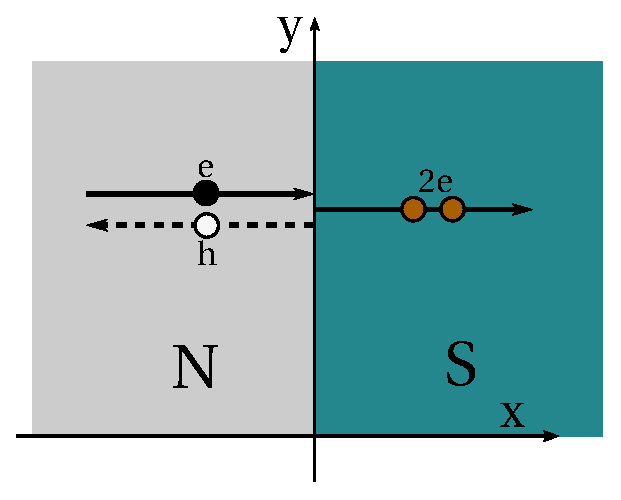
\includegraphics[width=0.5\textwidth]{figure/framework-analytical/ns-interface_csch}
\caption{Andreev reflection at an NS interface. An incoming electron is Andreev reflected into a hole with opposite momentum, and a Cooper pair condensates into the superconductor. The interface is modelled as a sharp edge.}\label{fig:ns-interface}
\end{figure}
How does the eigenvalue problem (\ref{eq:BdG-eq}) with the potential (\ref{eq:delta }) differ from a quantum mechanical step potential set-up? The formalism is virtually identical, but there is a subtle and important difference in the results. In the normal region, there are electrons, whereas in the superconducting regions, there is a condensate of Cooper pairs. A normal electron can be reflected at the interface as a hole and an additional Cooper pair can be created in the superconducting region (see figure \ref{fig:ns-interface}). By solving the Bogoliubov-de-Gennes equation in (\ref{eq:BdG-eq}), this picture becomes clearer.  This equation needs to be solved both for the normal and the superconducting region. When treating this problem quantum-mechanically, energies below and above the gap need to be considered independently. The resulting wave functions have to be continuous at the interface. Depending on the region, the gap parameter in the Hamiltonian in eq. (\ref{eq:H-BdG-r}) is either zero or $\Delta_0$.

\subsection*{Semi-classical Approximation: Andreev Equations}

With the NS interface, the gap parameter varies slowly over scales of $k_F^{-1}$, and it may vary over scales of the coherence length $\xi_0$. Because $k_F^{-1}$ is a good length scale for this problem, the equations above can be simplified:
\begin{equation}
\Psi \left( \mathbf{r} \right) = e^{i \mathbf{k_F} \mathbf{r} } \begin{pmatrix} u \left( \mathbf{r} \right) \\ v \left( \mathbf{r} \right)\end{pmatrix}.
\end{equation}
Since $u  \left( \mathbf{r} \right) $ and $v  \left( \mathbf{r} \right) $ vary slowly over distances of order $k_F^{-1}$, the second derivative with respect to $\mathbf{r}$ can be neglected. This approach is called the semi-classical approximation, which allows to transform the BdG eqs. (\ref{eq:BdG-eq})into the Andreev equations
\begin{eqnarray}
- i \hbar \mathbf{v}_F \nabla u \left( \mathbf{r} \right)  + \Delta \left( \mathbf{r} \right)  v  \left( \mathbf{r} \right)  &=& \epsilon u  \left( \mathbf{r} \right)  \\
 i \hbar \mathbf{v}_F \nabla v  \left( \mathbf{r} \right)  + \Delta^* \left( \mathbf{r} \right)  u  \left( \mathbf{r} \right)  &=& \epsilon v  \left( \mathbf{r} \right) .
\end{eqnarray}
These equations are significantly easier to handle than the BdG-equations, since they describe a first-order problem.

Consider an incoming particle from the left half-space $x < 0 $, travelling towards the superconducting interface at $x=0$, assuming that both the normal region and the superconductor have the same Fermi velocity $v_F$. The one-dimensional Andreev equations for the NS interface read
\begin{eqnarray}
- i \hbar v_{F, x} \frac{d}{d x} u \left( x \right)  + \Delta(x) v \left( x \right) &=& \epsilon u \left( x \right)\\
 i \hbar v_{F, x} \frac{d}{d x} v \left( x \right) + \Delta^*(x) u \left( x \right) &=& \epsilon v \left( x \right).
\end{eqnarray}
%\subsubsection*{Solution for the normal region}
In the normal region (for $x < 0$), the superconducting gap parameter decreases to zero on a length scale shorter than $\xi_0$. Therefore, the step-like approximation from eq. (\ref{eq:delta }) holds. In the normal region, 
the coefficients $u \left( x \right)$ and $v \left( x \right)$ are independent. The ansatz contains an incident wave with unity amplitude and a reflected hole with amplitude $r$. 
\begin{equation}
\Psi_N \left( x \right) = \begin{pmatrix} u \left( x \right) \\ v \left( x \right) \end{pmatrix}_N = e^{i k_N x } \begin{pmatrix} 1 \\ 0 \end{pmatrix} + r e^{-i k_N x } \begin{pmatrix} 0 \\ 1 \end{pmatrix},  \label{eq:psi-normal}
\end{equation}
where, writing $v_x \equiv v_{F, x}$, 
\begin{equation}
k_N = \frac{\epsilon}{\hbar v_x}.
\end{equation}
%TODO den Teil da unten wieder reinnehmen, wenn verstanden?
%\subsubsection*{Solution in the superconducting region}
In the superconducting region, the solution for the wave function has the form
\begin{equation}
\Psi_S \left( x \right) = \begin{pmatrix} u \left( x \right) \\ v \left( x \right) \end{pmatrix}_S = t e^{i k_S x } \begin{pmatrix} u_0 \\ v_0 \end{pmatrix}.
\end{equation}
The expression for the wave vector $k_S$ depends on the energy of the incoming particle, which can be either \emph{above} or \emph{below} the gap.\newline \newline
For high energies \emph{above} the gap,  $\epsilon > |\Delta|$ , the wave vector is
\begin{equation}
k_S = \frac{\sqrt{\epsilon^2 - \Delta^2}}{\hbar v_x}
\end{equation}
If the energy of the incoming particle is higher than the gap energy, it can be transmitted into the superconductor. The amplitude $t$ therefore is the transmission probability. The coherence factors $u_0$, $v_0$ can be found by solving the BdG equations within the BCS framework. Matching the boundary conditions at the interface yields
\begin{equation}
r = \frac{v_0}{u_0}, \quad t = \frac{1}{u_0}.
\end{equation}
Normalizing the wave functions leads to 
\begin{equation}
|r|^2 + (u_0^2 - v_0^2)|t|^2 = 1
\end{equation}
Since $\epsilon$ is the energy relative to the Fermi energy, the normal wave vector from eq. (\ref{eq:psi-normal}) can be written in terms of
\begin{equation}
\mathbf{q}_\pm =  \left( k_F \pm \frac{\epsilon}{\hbar v_F} \right) \hat{\mathbf{k}_F} \label{eq:q-pm}
\end{equation}
\begin{equation}
\Psi_N \left( \mathbf{r} \right) = e^{i\mathbf{q}_+ \cdot \mathbf{r}} \begin{pmatrix} 1 \\ 0\end{pmatrix} + a e^{i\mathbf{q}_- \cdot \mathbf{r}} \begin{pmatrix} 0 \\ 1\end{pmatrix}.
\end{equation}
Using eq. (\ref{eq:q-pm}), one can determine the trajectory of the reflected hole to coincide with the trajectory of the incoming electron. The change in momentum,
\begin{equation}
\Delta p_x = - \frac{2 e }{v_x},
\end{equation}
is small. The components $p_y$, $p_z$ are conserved, therefore the trajectory of the reflected hole is almost the same as the trajectory of the incoming electron. %TODO figure!
%In this solution, the incoming electron has the momentum 
%\begin{equation}
%q  = k_F + \frac{\epsilon}{\hbar v_F} \quad \rightarrow \epsilon(q) = \hbar v_F \left( q - k_F \right)
%\end{equation}
%with a positive group velocity $v_g = v_F$, whereas the reflected hole has the momentum
%\begin{equation}
%q  = k_F - \frac{\epsilon}{\hbar v_F} \quad \rightarrow \epsilon(q) = \hbar v_F \left( k_F - q \right)
%\end{equation} 
%with negative group velocity $v_g = - v_F$. \\


For energies \emph{below} the gap, $\epsilon < |\Delta |$, there are no states available inside the gap. Therefore, the wave function decays inside the superconductor. 

The wave function is
\begin{equation}
\begin{pmatrix} u\left(x\right) \\ v\left(x\right) \end{pmatrix}_S = t e^{- \tilde{k_S} x } \begin{pmatrix} u_0 \\ v_0 \end{pmatrix},
\end{equation}
where
\begin{equation}
\tilde{k}_S= \frac{\sqrt{\Delta^2 - \epsilon^2 }}{\hbar v_x}.
\end{equation}
For sub-gap energies, the amplitudes of the normal wave functions are slightly modified:
\begin{equation}
r = \frac{\tilde{v_0}}{\tilde{u_0}} 
\end{equation}
and
\begin{equation}
\text{and} \quad t = \frac{1}{\tilde{u_0}}, 
\end{equation}
where
\begin{equation}
\tilde{u_0} = \frac{1}{\sqrt{2}} \left( 1 + i \frac{\sqrt{|\Delta|^2 - \epsilon^2}}{\epsilon} \right) \quad \text{and} \quad \tilde{v_0} = \frac{1}{\sqrt{2}} \left( 1 - i \frac{\sqrt{|\Delta|^2 - \epsilon^2}}{\epsilon} \right).
\end{equation}
In this case, it holds that
\begin{equation}
|r|^2 = 1
\end{equation}
In other words, there are no transmitted particles and all particles are Andreev reflected.

\section{Theory Of SNS Junctions}\label{sec:theory-sns}
So far, only NS interfaces have been considered. The same procedure can be applied to superconductor - normal metal - superconductor (SNS) junctions: A sandwich structure of a superconductor on the left side, a normal region in the middle and a superconductor on the right side, as visualized in figure \ref{fig:sns-junction}. At both interfaces, a particle can be Andreev-reflected.
Each time an electron is Andreev-reflected at the right side and a hole travels back, a Cooper pair is induced into the right superconductor. In the same manner, a Cooper pair is stolen from the left superconductor when the hole is Andreev-reflected as an electron. This process is illustrated in figure \ref{fig:sns-junction}. As an overall consequence, a supercurrent through the SNS junction can be observed. This process leads to localized electrons with bound states, known as Andreev bound states.
\begin{figure}
\centering
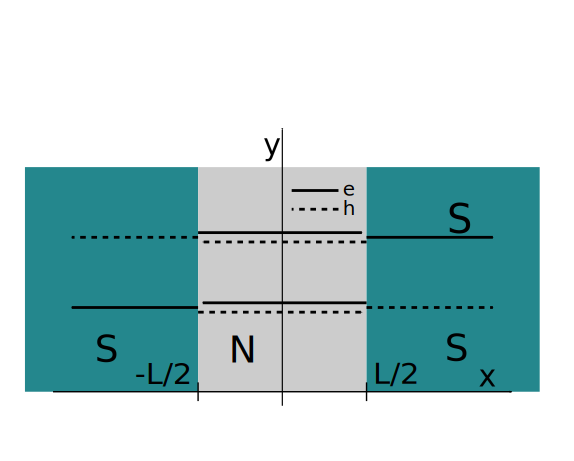
\includegraphics[width=0.5\textwidth]{figure/framework-analytical/sns_csch}
\caption{An SNS junction of width $W$. Electrons are indicated as solid arrows, holes as dashed ones. An electron (hole) is Andreev reflected as a hole (electron) at one side, which then again is reflected at the other side. In this way, Andreev bound states form in the junction.}\label{fig:sns-junction}
\end{figure}


In the following, an SNS junction with normal region at $|x| < W/2$, the right superconductor at $x > + W/2$ and the left superconductor at $x < -W/2$ is considered. The electrons in both superconducting regions and in the normal metal have the same Fermi velocity and there are no insulating barriers between them. This means that $W$  is smaller than the electron mean free path. For short $W$ this implies that the mean free path is larger than the superconducting coherence length. The phase difference between the superconductors is $\chi$, so the right superconductor can be assumed to be characterised by the phase $\chi/2$ and the left one by $-\chi/2$. 
The semi-classical approximation is used and a wave function with the form
\begin{equation}
\Psi \left( \mathbf{r} \right) = e^{i \mathbf{k_F} \mathbf{r} } \begin{pmatrix} u \left( \mathbf{r} \right) \\ v \left( \mathbf{r} \right)\end{pmatrix}.
\end{equation}
is needed. 
In the normal region, it holds that 
\begin{eqnarray}
\Psi_N \left( x \right) &=& A\cdot \left[ e^{i k_N x } \begin{pmatrix} 1 \\ 0 \end{pmatrix} + a e^{-i k_N x } \begin{pmatrix} 0 \\ 1 \end{pmatrix} \right], \label{eq:sns-psi-normal}\\
k_N &=& \frac{\epsilon}{\hbar v_x}.
\end{eqnarray}
Assuming that $k_x > 0$, the wave function in the right superconductor ($x > W/2$) is
%\begin{pmatrix} u \left( x \right) \\ v \left( x \right) \end{pmatrix}_R 
\begin{eqnarray}
\Psi_S^R \left( x \right) &=& d_1 e^{ - \tilde{k}_S x } \begin{pmatrix} \tilde{u}_0 e^{i \chi/4} \\ \tilde{v}_0 e^{-i \chi/4} \end{pmatrix},\\
\tilde{k}_S  &=& \frac{\sqrt{|\Delta|^2 - \epsilon^2 }}{\hbar |v_x|}.
\end{eqnarray}
For the left superconductor, the wave function is
\begin{equation}
 \Psi_S^L \left( x \right) = d_1' e^{ \tilde{k}_S x } \begin{pmatrix} \tilde{v}_0 e^{-i \chi / 4}\\ \tilde{u}_0 e^{i \chi / 4} \end{pmatrix}.
\end{equation}
Applying the continuity condition at the interfaces leads to
\begin{eqnarray}
a e^{-i k_n W} &=& \frac{\tilde{v}_0}{\tilde{u}_0} e^{-i \chi /2}  \\
a e^{i k_n W} &=& \frac{\tilde{u}_0}{\tilde{v}_0} e^{i \chi /2}.
\end{eqnarray}
Combining these equations, we find
\begin{equation}
e^{2i ( k_N W - \chi /2 )}  = \frac{\epsilon + i \sqrt{|\Delta|^2 - \epsilon^2 }}{ \epsilon - i \sqrt{|\Delta|^2 - \epsilon^2 } } \label{eq:energy-exp}.
\end{equation}
To simplify this expression, one can introduce 
\begin{equation}
\sin \alpha := \frac{\epsilon}{|\Delta|}, \quad - \pi / 2 < \alpha < \pi / 2\label{eq:sinalpha}
\end{equation}
Using eq. (\ref{eq:sinalpha}), one can rewrite the right hand side of eq. (\ref{eq:energy-exp}) in terms of trigonometric functions and gets
\begin{equation}
e^{2i ( k_N W - \chi /2 )} = e^{-2i \alpha + i \pi},
\end{equation}
which then leads to
\begin{equation}
\epsilon = \frac{\hbar v_x}{W} \left( \pi \left(l + \frac{1}{2} \right) - \arcsin \frac{\epsilon}{|\Delta|} + \frac{\chi}{2} \right).
\end{equation}
%TODO short summary, what has been done up to this point?
If $k_x < 0 $, it holds that
\begin{equation}
\Psi_S^R \left( x \right) = d_2 e^{ - \tilde{k}_S x } \begin{pmatrix} \tilde{v}_0 e^{i \chi/4} \\ \tilde{u}_0 e^{-i \chi/4} \end{pmatrix}
\end{equation}
For the left superconductor, the wave function is
\begin{equation}
\Psi_S^L \left( x \right)  = d_2' e^{ \tilde{k}_S x } \begin{pmatrix} \tilde{u}_0 e^{-i \chi / 4}\\ \tilde{v}_0 e^{i \chi / 4} \end{pmatrix}
\end{equation}
An analogous calculation leads to
\begin{equation}
\epsilon = - \frac{\hbar |v_x|}{W} \left( \pi \left(l - \frac{1}{2} \right) + \arcsin \frac{\epsilon}{|\Delta|} + \frac{\chi}{2} \right)
\end{equation}
The final result for the spectrum is
\begin{equation}
\epsilon = \pm \frac{\hbar |v_x|}{W} \left( \pi \left(l \pm \frac{1}{2} \right) \mp \arcsin \frac{\epsilon}{|\Delta|} + \frac{\chi}{2} \right)
\end{equation}
The upper sign is corresponds to $k_x > 0$ and the lower sign corresponds to $k_x  <0 $.\\
Normalizing the wave functions fixes the coefficient in eq. (\ref{eq:psi-normal})
\begin{equation}
|A|^2 = \frac{1}{2(W+ k_S^{-1})} = \frac{1}{2} \frac{\sqrt{|\Delta|^2 - \epsilon^2}}{\hbar |v_x| + W \sqrt{|\Delta|^2 - \epsilon^2}}.
\end{equation}
%TODO maybe a bit more how |A|^2 is calculated?
\subsubsection*{Limit of short junction}

For junctions with small width $W$, such that 
\begin{equation}
W \ll \frac{\hbar v_x }{|\Delta|}, \quad \xi \ll W
\end{equation}
holds, where $\xi_0 \sim \hbar v_F / |\Delta|$ is the coherence length. Then, in eq. (\ref{eq:energy-exp}) the term with $e^{2i k_n W} \approx 1$ and the spectrum becomes
\begin{equation}
\epsilon = \mp \cos \frac{\chi}{2}, \quad 0 < \chi < \pi.
\end{equation}

\subsubsection*{Limit of long junction}

Long junction, $W \gg \xi_0$, it holds that 
\begin{equation}
W \gg \frac{\hbar |v_x|}{|\Delta|}.
\end{equation} 
Then the spectrum is given by
\begin{equation}
\epsilon = \pm \frac{\hbar |v_x|}{W}\left(\frac{\chi}{2} - \frac{\pi}{2} \right) + \frac{l \pi \hbar |v_x|}{W},
\end{equation}
because $\arcsin \frac{\epsilon}{|\Delta|}$ can be neglected.


%\section{Supercurrent Through The SNS Junction}
%Having established the normal wave functions for SNS junctions, the quantum-mechanical current can be calculated. It is given by
%\begin{equation}
%\mathbf{j} = \frac{e}{m} \left[ f_n u_n^* \left( \mathbf{r} \right) \left( - i \hbar \nabla - \frac{e}{c} \mathbf{A} \right) u_n\left( \mathbf{r} \right) + \left(1-f_n\right) v_n\left( \mathbf{r} \right) \left( -i \hbar \nabla - \frac{e}{c} \mathbf{A} \right) v_n^*\left( \mathbf{r} \right) + \text{c.c.} \right], \label{eq:current-qm}
%\end{equation}
%where $n$ labels quantum states and $f_n$ is the corresponding Fermi distribution.
%As a simplification, $\mathbf{A} = 0$ is considered:
%\begin{equation}
%\mathbf{j} = - i \hbar  \frac{e}{m} \left[ f_n u_n^* \left( \mathbf{r} \right) \nabla  u_n \left( \mathbf{r} \right) + \left(1-f_n\right) v_n\left( \mathbf{r} \right) \nabla v_n^*\left( \mathbf{r} \right) + \text{c.c.} \right].
%\end{equation}

%For evaluating eq. (\ref{eq:current-qm}), the normal wave functions from eq. (\ref{eq:sns-psi-normal}) are used. In the semi-classical approximation, only the derivatives of the rapidly varying functions $e^{i\mathbf{k r}}$ contribute to the current, which then reduces to
%\begin{equation}
%I_x = - \frac{e}{\hbar} \sum_n \left(1- 2 f_n \right) \frac{\hbar v_x \sqrt{|\Delta^2| - \epsilon_n^2}}{\hbar v_x + W \sqrt{|\Delta|^2 -\epsilon^2}}.
%\end{equation}

\section{SNS Junction And The Josephson Effect}
The Josephson effect \cite{Josephson1962} describes the flow of a supercurrent through two superconducting leads coupled by a weak link. This weak link can be an insulator or a normal conductor. The conventional picture is that the current can be described as a consequence of Cooper pairs tunneling through a barrier. It is also possible to view the current as a consequence of electrons being Andreev reflected, as has been described in section \ref{sec:theory-sns} from one superconducting leads. The bound states, that from in the junction carry the current from one superconductor to another. A calculation of the Josephson current within the framework presented above, i.e. starting with the BdG Hamiltonian and matching the wave functions at the interface, is presented in \cite{Furusaki1999}.
%TODO maybe add the short and long junction limit results?
Within the picture of electrons tunnelling through a barrier, the supercurrent density is found from the generalized London equation
\begin{equation}
\mathbf{J}_s ( \mathbf{r}, t ) = q_s n_s (\mathbf{r}, t ) \left( \frac{\hbar}{m_s} \nabla \chi (\mathbf{r}, t ) - \frac{q_s}{m_s} \mathbf{A} \right) \equiv \frac{q_s n_s \hbar}{m_s} \mathbf{\gamma} (\mathbf{r}, t ),\label{eq:current-density-general}
\end{equation}
where $q_s$ are the chare carriers in a superconductor ($q_s = 2e$) and $n_s$ is the density of the superconducting electrons. The supercurrent density is a function of $\chi$. It has a $2 \pi$-periodicity and it is zero for $\chi = 0$:
\begin{eqnarray}
J_s ( \chi)  &=& J_s ( \chi  + n 2 \pi) \\
J_s ( \chi = 0 ) &=& J_s ( \chi = n \cdot 2\pi) = 0
\end{eqnarray}
Therefore, the most general solution for the supercurrent density is of the form
\begin{equation}
J_s (\chi) = J_c \sin \chi + \sum_{m=2}^{\infty} J_m \sin(m \chi),
\end{equation}
where $J_c$ is the critical Josephson current density. In most cases however, it is sufficient to only consider the first term, so that
\begin{equation}
J_s ( \chi ) = J_c \sin \chi
\end{equation}
When including a magnetic field, the phase will become a function of the vector potential $\mathbf{A}$. By calculating the phase difference $\chi(y_A) - \chi (y_B)$ of two points $y_A$, $y_B$ along the $y$-axis the effect of the magnetic field to the Josephson relation can be determined.
Using eq. \ref{eq:current-density-general}:
\begin{eqnarray}
\tilde{\chi}(\mathbf{r}) &=& \int _1^2 \mathbf{\gamma (\mathbf{r})} = \int_1^2 \left( \nabla \chi (\mathbf{r}) - \frac{2 \pi}{\phi_0} \mathbf{A} \right) \cdot d \mathbf{l}\\
 &=& \chi_2 - \chi_1 - \frac{2 \pi}{\phi_0} \mathbf{A} \cdot d \mathbf{l} \\
% &=& \chi - \frac{2 \pi}{\phi_0} \int{-L/2}^{+L/2} (-By) dx \\
 &=& \chi - \frac{2 \pi}{\phi_0}B L y
\end{eqnarray}
This leads to the current density 
\begin{equation}
J_s = J_c \sin ( \chi - \frac{2 \pi}{\phi_0}B L y) = J_c \sin ( \chi - \frac{2 \pi \phi}{W \phi_0} y)
\end{equation}
Integration over x leads to
\begin{equation}
\int dy J(y) = \int_0^W J_c  \sin ( \chi - \frac{2 \pi}{\phi_0}B L y) = J_c \frac{W \phi_0}{2 \pi \phi} ( \cos (\chi_0) - \cos ( 2 \pi \phi / \phi_0 + \chi_0 ) )
\end{equation}
Maximising the above equation with respect to $\chi$ gives the critical current
\begin{equation}
I_c = W J_c \left| \frac{\sin (\pi \phi / \phi_0)}{\pi \phi / \phi_0} \right|
\end{equation}
\section{Graphene And Superconductivity: Specular Andreev Reflection}
An unusual form of Andreev reflection has been found at graphene - superconductor interfaces \cite{Beenakker2006}. The previously discussed Andreev reflection changes the direction of the incoming particle such that the reflected particle travels on approximately the same trajectory as the incoming one (see section \ref{sec:NS}). This process is called Andreev retro reflection and is illustrated in figure \ref{fig:specular-sns} b. It is only an approximation, because due to its condensation into a cooper pair, the particle will lose energy during the reflection process. In most metals, hardly any energy loss is observed because the Fermi energy of most metals is large compared to the superconducting energy gap, $E_F \gg \Delta$ \cite{Efetov2016}. Graphene, however, is a semi-metal with low $E_F$, where the regime with $E_F < \Delta$ is achievable. As a consequence, the $E_F$ dependence of Andreev reflection can be studied in graphene. \\
The single-particle Hamiltonian for graphene is the Dirac Hamiltonian
\begin{equation}
H = \begin{pmatrix}
H_+ & 0 \\
0 & H_- 
\end{pmatrix},
\end{equation}
where
\begin{equation}
H_\pm = i \hbar \left( \sigma_x \delta_x \pm \sigma_y \delta_y \right) + U.
\end{equation}
For the expression of $H_\pm$, the pauli matrices $\sigma_i$ have been used. An electrostatic potential, $U(\mathbf{r})$, can be present in the sample. Here, it is chosen such that
\begin{equation}
U(\mathbf{r}) = -U_0 \theta (x)
\end{equation} 
This modifies the BdG equation, resulting in 
\begin{equation}
\begin{pmatrix}
H_\pm + E_F & \Delta \\
\Delta^* & E_F - H_\pm 
\end{pmatrix} \begin{pmatrix}
u \\ v \end{pmatrix} = \epsilon \begin{pmatrix} u \\v \end{pmatrix}, \label{eq:dirac-hamiltonian}
\end{equation}
where the electron spinor has two components $\begin{pmatrix} u_1, u_2\end{pmatrix} = \begin{pmatrix} \Psi_{A+}, \Psi_{B+} \end{pmatrix}$, and the hole spinor is $\begin{pmatrix} v_1, v_2\end{pmatrix} = \begin{pmatrix} \Psi^{*}_{A-},  \Psi^{*}_{B-} \end{pmatrix}$.
Eq. (\ref{eq:dirac-hamiltonian}) leads to the energy spectrum
\begin{equation}
\epsilon = \sqrt{|\Delta|^2 + \left( E_F - U \pm \hbar v |\mathbf{k}|\right) ^2},  
\end{equation}
with
\begin{equation}
|\mathbf{k}| = \sqrt{k_x^2 + k_y^2}.
\end{equation}
The dispersion relation has four solutions for $\mathbf{k}$. Two of them lead to a positive velocity $v_x = \hbar^{-1} d \epsilon d k_x$ corresponding to each one electronic and one hole excitation. A reflected hole can be in one of the following two states: It is reflected either into the conduction band with $\epsilon < E_F$ (retro reflection) or into the valence band with $\epsilon > E_F$ (specular reflection). Specular reflection is the dominating process, when the Fermi energy is smaller than the gap energy, $E_F \ll \Delta$. For $E_F \gg \Delta$, the retro reflection dominates. 
\begin{figure}
\centering
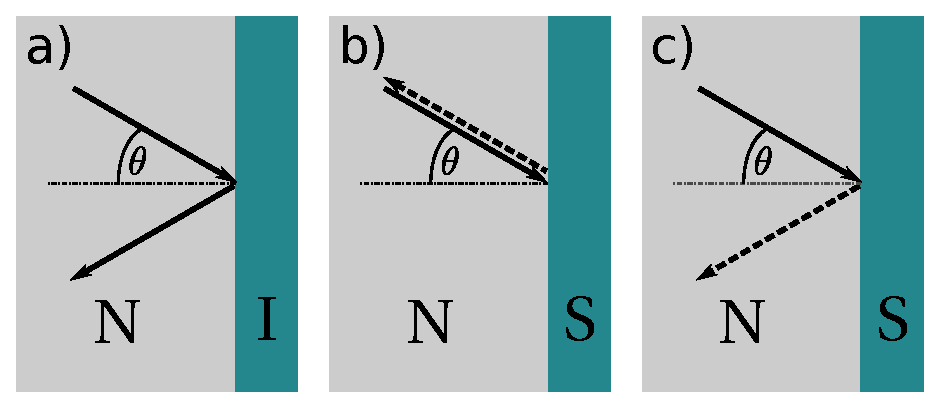
\includegraphics[width=0.7\textwidth]{figure/framework-analytical/specular-reflection_csch}
\caption{Reflection processes. Solid arrows represent electrons, dashed arrows represent holes. \\ a) Specular reflection of an electron at an insulating interface (I). \\ b) Andreev retro reflection of an electron with into a hole. \\ c) Specular Andreev reflection of an electron into an hole with incident angle $\theta \neq 0$.}\label{fig:specular-sns}
\end{figure}

 
